% Reproduction Slides

\begin{frame}{Vision Results: Regularization Induces Low-Rank Structure}
    \begin{columns}
        \column{0.5\textwidth}
        \textbf{Key Finding:}
        \begin{itemize}
            \item Effective rank: \textbf{15.5} (WD) vs \textbf{38.5} (none)
            \item Ratio: \textbf{0.40} $<$ 0.5 \checkmark
            \item Accuracy: \textbf{97--98\%}
        \end{itemize}
        
        \vspace{0.2cm}
        \textbf{Main Driver:}
        \begin{itemize}
            \item Weight decay drives low-rank structure
            \item Noise improves accuracy but increases rank
            \item WD alone achieves lowest effective rank
        \end{itemize}
        
        \vspace{0.2cm}
        \textbf{Claim V1:} Fully reproduced \checkmark
        
        \column{0.5\textwidth}
        \begin{figure}
            \centering
            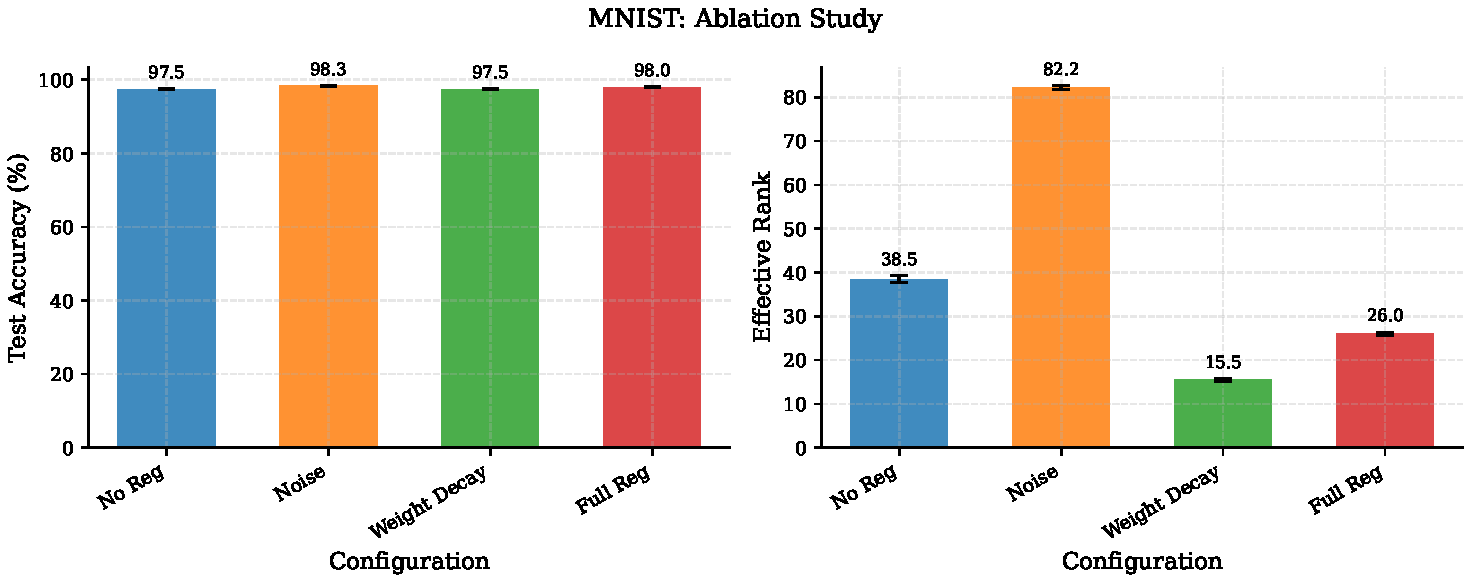
\includegraphics[width=0.95\textwidth]{../Report/figures/vision/mnist_ablation.pdf}
            \caption{Accuracy vs.\ effective rank}
        \end{figure}
    \end{columns}
\end{frame}

\begin{frame}{Vision Results: Interpretable Eigenvectors}
    \begin{columns}
        \column{0.5\textwidth}
        \textbf{Regularized Models:}
        \begin{itemize}
            \item Clear digit patterns
            \item Recognizable stroke templates
            \item Interpretable geometric features
        \end{itemize}
        
        \vspace{0.2cm}
        \textbf{Unregularized Models:}
        \begin{itemize}
            \item Diffuse, noise-like patterns
            \item No clear structure
            \item Overfitting to training data
        \end{itemize}
        
        \vspace{0.2cm}
        \textbf{Claims V2 \& V3:} Fully reproduced \checkmark
        
        \column{0.5\textwidth}
        \begin{figure}
            \centering
            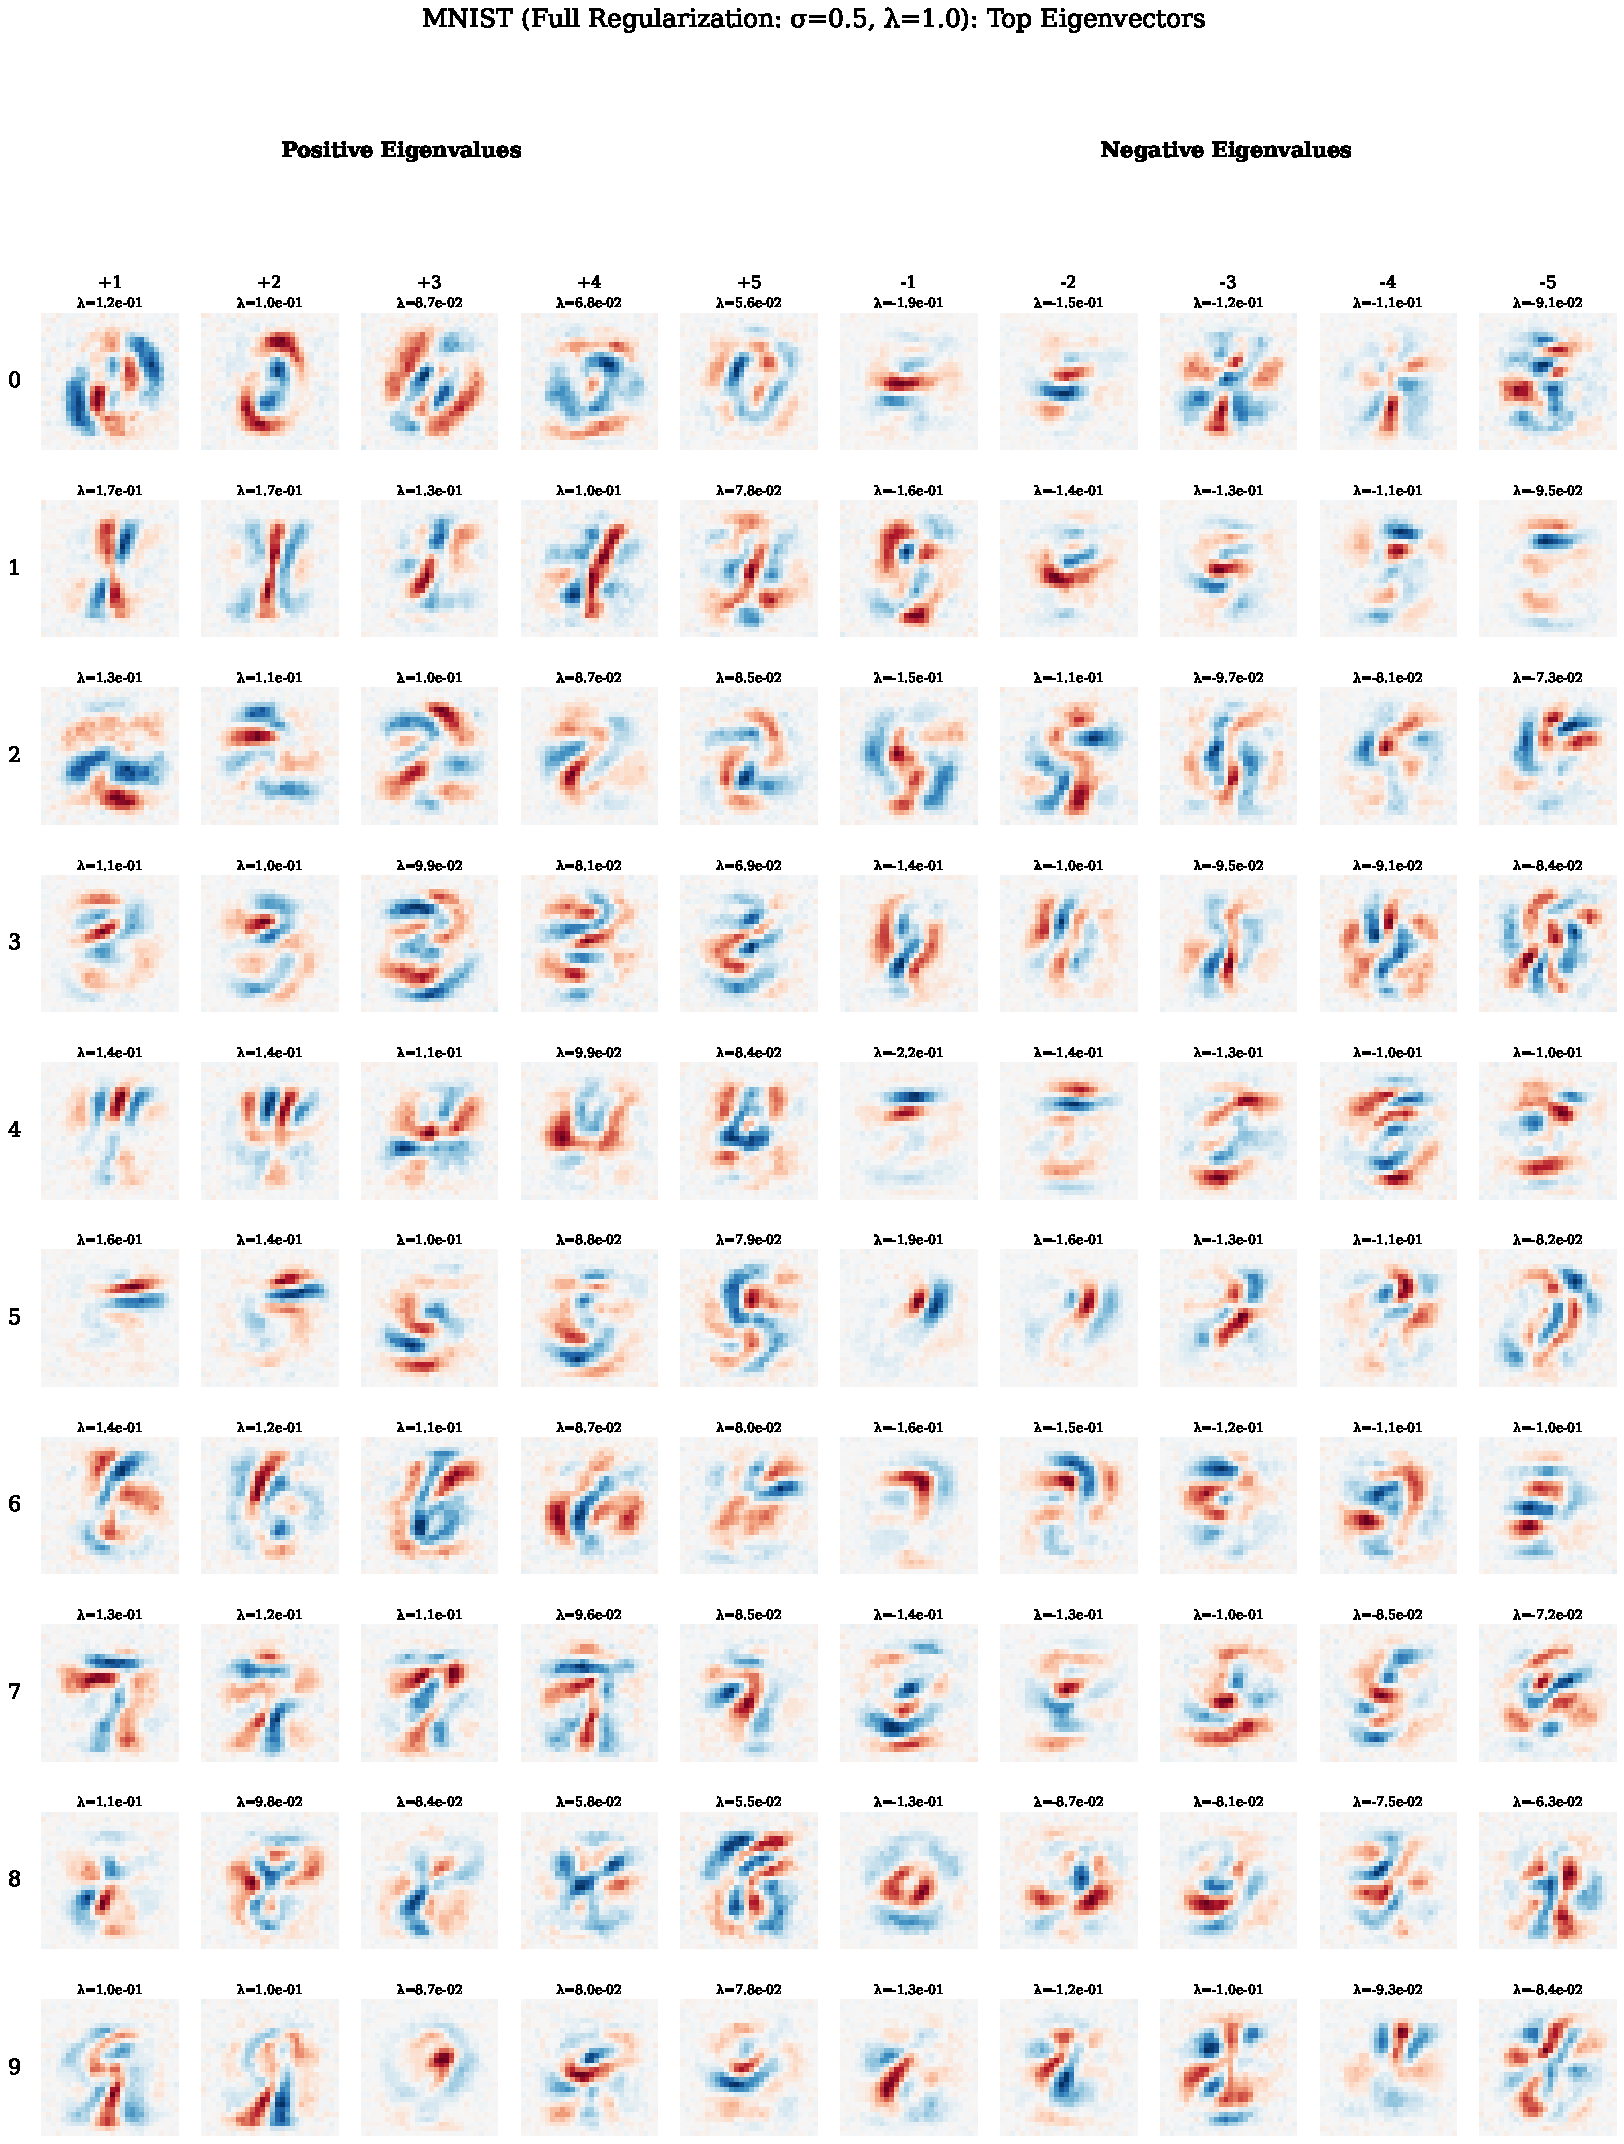
\includegraphics[width=0.95\textwidth]{../Report/figures/vision/eigenvectors_reg.pdf}
            \caption{Regularized eigenvectors (top 10 per class)}
        \end{figure}
    \end{columns}
\end{frame}

\begin{frame}{Language Results: Negation Circuit Discovery}
    \begin{columns}
        \column{0.5\textwidth}
        \textbf{AND-Gate Circuit:}
        \begin{itemize}
            \item Feature 751: strongest AND-gate
            \item AND-score: \textbf{0.96}
            \item Eigenvalues: $\lambda_1 = -0.46$, $\lambda_2 = +0.18$
        \end{itemize}
        
        \vspace{0.2cm}
        \textbf{Semantic Structure:}
        \begin{itemize}
            \item \textbf{Positive:} ``wonderful'', ``excellent'', ``fortunate''
            \item \textbf{Negative:} ``horrible'', ``disease'', ``unfair''
            \item Clear block structure
        \end{itemize}
        
        \vspace{0.2cm}
        \textbf{Claims L1 \& L2:} Fully reproduced \checkmark
        
        \column{0.5\textwidth}
        \begin{figure}
            \centering
            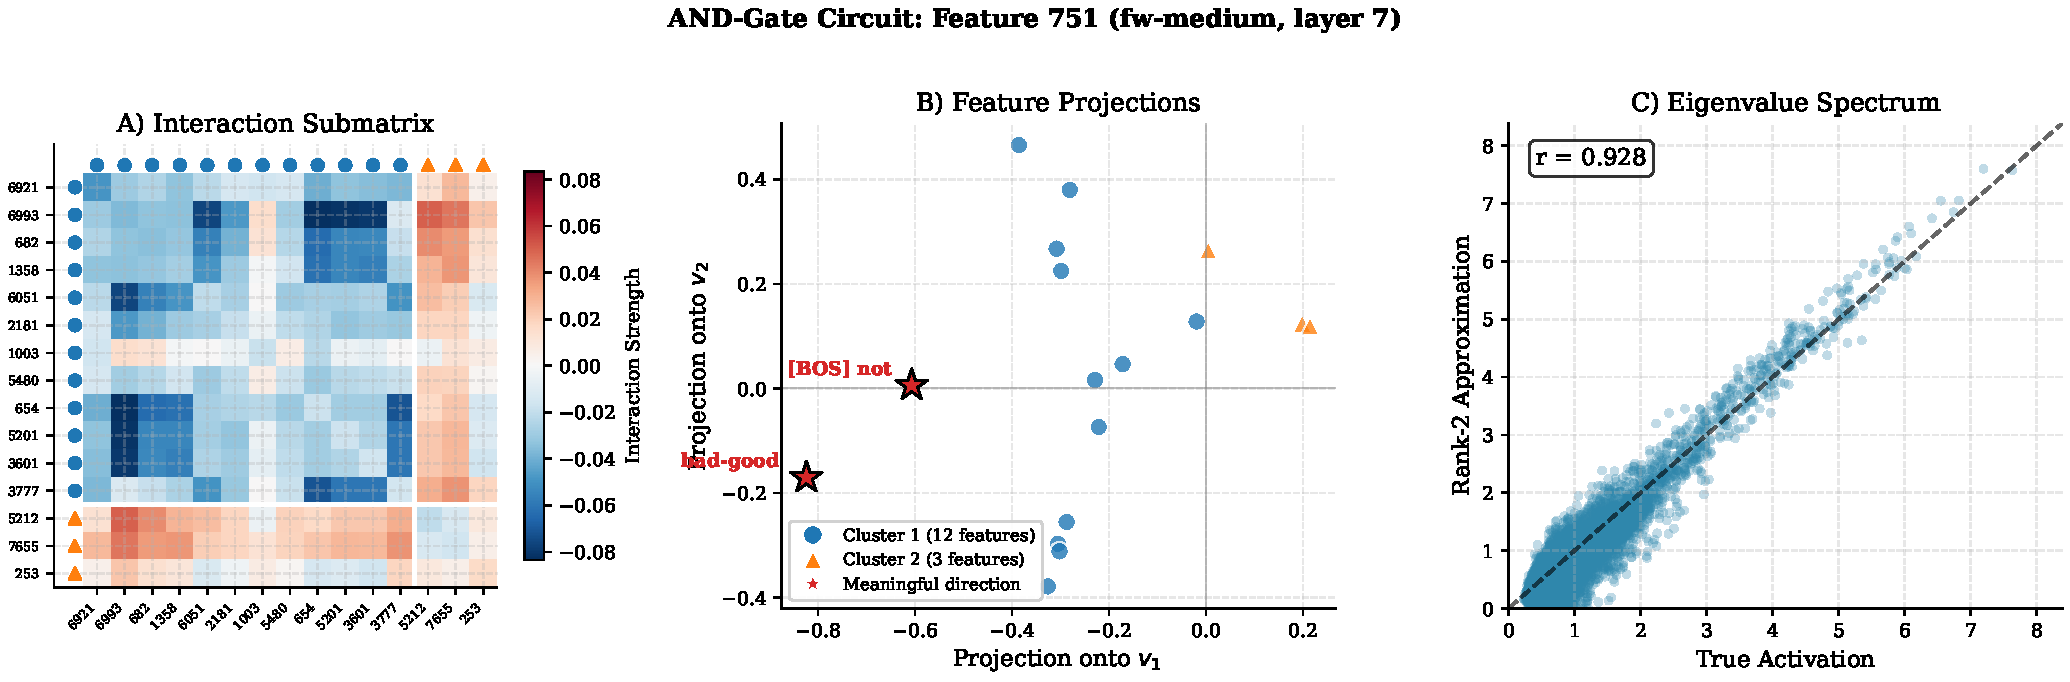
\includegraphics[width=0.95\textwidth]{../Report/figures/language/figure_8_feature751.pdf}
            \caption{Negation circuit: Feature 751}
        \end{figure}
    \end{columns}
\end{frame}

\begin{frame}{Language Results: Correlation Gap \& Root Cause}
    \begin{columns}
        \column{0.5\textwidth}
        \textbf{Claim L3:} 69\% achieve $>$0.75 rank-2 correlation
        
        \vspace{0.2cm}
        \textbf{Our Result:}
        \begin{itemize}
            \item Only \textbf{18--32\%} achieve $>$0.75
            \item Mean correlation: 0.27--0.51
            \item Significant gap from claim
        \end{itemize}
        
        \vspace{0.2cm}
        \textbf{Root Cause:}
        \begin{itemize}
            \item SAE training duration
            \item Correlation improves \textbf{2.5$\times$} with longer training
            \item Public SAEs less trained than paper's internal checkpoints
        \end{itemize}
        
        \footnotesize
        Methodology sound; gap from SAE quality
        
        \column{0.5\textwidth}
        \begin{figure}
            \centering
            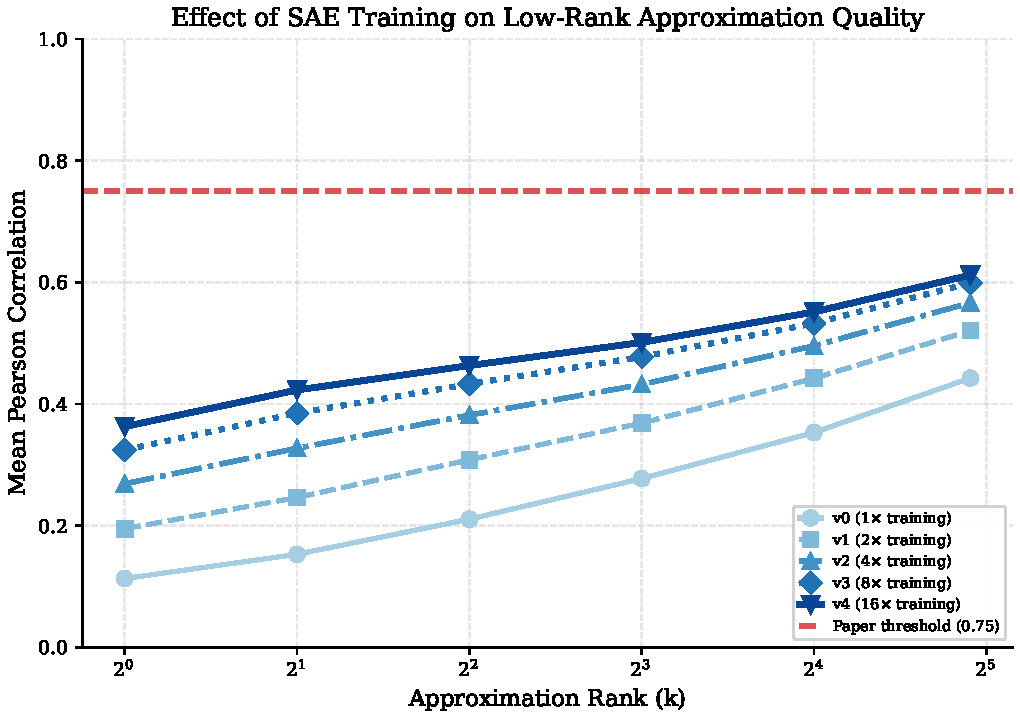
\includegraphics[width=0.95\textwidth]{../Report/figures/language/figure_10a_sae_training_effect.pdf}
            \caption{Correlation progression with SAE training}
        \end{figure}
    \end{columns}
\end{frame}
